\documentclass[12pt, a4paper]{article}
\usepackage{amssymb}
\usepackage{rotating}
\usepackage{cite}
\usepackage{amsmath}
\usepackage{listings}
\usepackage{url}
\usepackage{graphicx}
\usepackage{multirow}
\usepackage{media9}
\graphicspath{{../Figures/}}


\renewcommand{\thesection}{\arabic{section}}

\begin{document}

%%Title page
\begin{titlepage}

\centering
\Large

~\vspace{\fill}

{\huge 
Implementing 2D SIMBICON Using PyBullet
}

\vspace{1.5cm}

{\LARGE
Kaitlin Thachuk
}

\vspace{3.0cm}

A thesis submitted in partial fulfillment for the\\
degree of Bachelors of Science (Honours)\\[1em]
in the\\[1em]
Department of Computer Science\\[1em]
University of British Columbia

\vspace{3.0cm}

Supervisor: Prof. Michiel van de Panne

\vspace{\fill}

April 2018\\
\vspace{1.5cm}
{\small \copyright 2018\\
Kaitlin Thachuk\\
ALL RIGHTS RESERVED}
\end{titlepage}
%%%%
\begin{titlepage}


\begin{abstract}
This project explores locomotion of a biped in 2D using the SIMBICON (simple biped locomotion control) framework. It is meant to be an introduction to the field of physics-based character animation. The project is completed in a newer physics engine PyBullet and the character is represented using MuJoCo XML. The SIMBICON framework includes implementing a basic finite state machine comprised of four states which drive the walking motion of the character. Balance feedback, torso control using the stance leg torque, and ensuring the swing foot placement is unaffected by torso pitch all contribute to achieving a more balanced walk. Torques for all the joints are calculated using proportional-derivative (PD) controllers. Debugging these types of systems often involves many hours of manually searching a parameter space since PyBullet does not have any useful built in tools. The results of this project are a set of target angles, feedback parameters, and gain parameters which are utilized in the main program to produce a character that walks on a plane. These parameters are different from the ones found in the original SIMBICON paper which implies these values may be sensitive to the simulator and character representation used. 
\end{abstract}
\end{titlepage}
\newpage

\section*{Acknowledgements}
First and foremost thank you to Prof. Michiel Van de Panne for taking me on and sharing his time and knowledge to introduce me to this topic.\\

A special thank you to Kristen Ruhnke without whom this thesis would probably not have been written in any sort of reasonable time frame; your support and motivation have made all the difference.\\

Finally thank you to my parents who have offered endless encouragement over the years.
\newpage

\pagenumbering{roman}
\tableofcontents
\newpage
\listoffigures
\newpage
\listoftables

\newpage
\section{Introduction}
\pagenumbering{arabic}

\subsection{Previous Works}

The field of physics-based character animation has seen lots of improvement in the past ten years. Physics-based character animation is characterized by controlling the character through external forces and torques, meaning the global position and alignment of the character is not directly controllable \cite{Geijtenbeek}. This is contrasted by the much more popular in industry kinematics-based animation which concerns itself only with motion trajectories on which the characters move \cite{walking_survey}. The main problem with kinematics-based animation, and the main motivation for research into physics-based animation is that characters on a motion trajectory have no concept of mass, forces, or collision/object interaction dynamics \cite{walking_survey}. All these shortcomings are easily rectified if the character exists in a physics-based environment where interactions would naturally be in accordance with the laws of physics. Of course physics-based animation is not without its' own flaws and limitations. The major ones that have held it back thus far are the fact that controlling the characters is quite complex, requires a lot of manual tuning, and is prone to exhibiting erratic behaviours if the character loses control \cite{Geijtenbeek}. \\

Geijtenbeek summarized previous work in this field quite nicely in his 2012 paper \cite{Geijtenbeek} which I will abbreviate here. Physics simulators, which are used to produce physics-based character animation, at a high level perform three basic steps. The first is collision detection, which is looking for intersections in the geometries of objects. Collision detection itself is a vast field of study which is outside the scope of this project. For interested readers Fares and Hamam \cite{fares2005collision} 
wrote a state-of-the-art review on collision dynamics for rigid bodies which nicely summarizes some of the techniques in the field. The second step is forward dynamics simulation where laws of physics are applied to  caluculate the linear and angular acceleration produced by the forces \cite{walking_survey}. Finally the last step is numerical integration. Using the previously computed accelerations the positions, orientations, and velocities of the objects are updated. Again there has been some effort put into finding robust integration methods, one of which is the Runge Kutta method. Some examples of physics simulators/engines include Bullet and it's python wrapper PyBullet \cite{pybullet}, MuJoCo \cite{mujoco}, and Open Dynamics Engine (ODE) \cite{ode}.\\ 

Moving on to the character itself, often the character models are constrained rigid bodies. This indicates that their bodies are non-penetrable and non-elastic, and that their motion is constrained through limits on the joints connecting the links \cite{Geijtenbeek}. 
The joint constraints are meant to mimic the real life joint constraints experienced in humanoids, which the characters are often modelled after. The links themselves are often represented by simple geometries such as rectangles or cylinders, for which collision detection is easier, with given densities or masses which will be used by the forward dynamics step. The joints can be represented in many different ways, but the most common joints are hinge joints which could be used to model a knee or elbow joint, and ball-and-socket joint which would be useful for shoulders and hips.\\

Now that we have a basic understanding of how the character has been put together and the environment it will be in we can begin to discuss the real meat of the problem: motion control. A motion controller is responsible for helping the character achieve its' task like walking. There are three common design approaches to motion control: dynamics-based optimization control, stimulus-response network control and pose-driven feedback control \cite{Geijtenbeek}. Dynamics-based optimization control uses the equations of motion for the constrained dynamics to find joint torque vales that optimize a high level objective \cite{dynamics_control}. Stimulus-response network control has roots in AI and biological systems where a generic control network achieves motion control by constructing relations between the input sensors and the output joint torques \cite{Geijtenbeek}. The design technique used in this project is pose-driven feedback, where the character has a set of target angles that form a pose and feedback controllers are used to compute torques that minimize the difference between the current pose and the target pose \cite{walking_survey}. \\

Feedback controllers are another area where there are quite a few different methods being used to control the character. For the sake of brevity, the focus will be on the ones used in this project although a more extensive list can be found in Geijtenbeek \cite{Geijtenbeek}. The control technique utilized in this paper is called proportional-derivative (PD) control, which computes a torque that is linearly proportional to the difference between the current orientation and velocity and the desired orientation and velocity \cite{walking_survey}. The equation governing this control method is 

\begin{equation}
\tau = k_p(\Theta_d - \Theta) + k_d(\dot\Theta_d -\dot\Theta),
\label{eqn: pd control}
\end{equation} 
\noindent
where $\tau$ is the calculated torque, $\Theta$ and $\dot\Theta$ represent the position and velocity of the joint, the subscript $d$ indicates desired values for the position and velocity and $k_p$, $k_d$ are controller gain values.\\

To actually get a character to perform an action such as walking we need to move through a progression of poses. The most general way this can be achieved is by using a finite state machine in which each state is associated with a key target pose \cite{Geijtenbeek}. Common triggers for state transitions are time limits and foot contacts. It is important to note that these target poses might not actually be reached when simulating and that some exaggeration might be necessary to achieve the desired motion. While this strategy is effective for 2D characters when moving in 3D some additional control is required for dealing with balance. The 3D implementation is outside the scope of this project so refer to \cite{Yin07} for more details.  

\subsection{Overview of Approach}
Animating walking humanoids has long been both a challenging and crucial problem in compute graphics \cite{walking_survey}. The simple biped locomotion control (SIMBICON) framework \cite{Yin07} aims to take the generally unstable biped and apply balance and feedback laws to create more robust motion.  The purpose of this project was to reimplement the work done by Yin et al. \cite{Yin07} on SIMBICON in 2D using a newer physics simulator, PyBullet. SIMBICON is a framework for controlling a biped in both 2D and 3D using a pose-control finite state machine. This allows for a large flexibility in the amount of gaits possible and makes it possible to transition between gaits smoothly. In each state we apply torques to the joints that are calculated using PD controllers. Finally balance control is provided in the form of a feedback strategy that attempts to place the foot appropriately given the position of the body's center of mass as well as feedback to try and keep the torso upright.  

\newpage
\section{Methods}
Some of the methods (Secs. 2.1-2.3) described in this paper are techniques taken from the Yin et al. \cite{Yin07}. 
\subsection{Finite State Machine}
As mentioned above the character is controlled using a finite state machine. Each state has its own target pose which is given as a set of target joint angles for the stance and swing legs. The stance leg is the leg that remains in contact with the ground and provides stability whereas the swing leg is in motion driving towards the desired pose. The torques for each state are computed for each joint using Eq. \ref{eqn: pd control} and the target angles for that particular state. The torques are continually updated while in a given state until a state transition occurs. The states are also symmetric with respect to left and right. \\ 

Fig. \ref{fig: finite state} shows a visual representation of the figure moving through the four states and we can see before the finite state machine starts the figure begins in a neutral position standing on the plane. Then in state 0 the right foot begins to swing forward trying to achieve its' desired pose. After 0.3sec we transition to state 1 where the right leg is still the swing leg but now the leg is coming down towards the plane. When the right foot makes contact with the ground we transition to state 2 which is a mirror image of state 0. In this state we now have the left leg as the swing leg and it is driving forward. After 0.3sec we again transition to state 3 which is the mirror of state 1. In this state we have the left leg driving down towards the ground and when the left foot makes contact we will transition back to state 0 and repeat the cycle. Table \ref{fig: finite state} contains a summarized version of the swing and stance legs as well as the transition for each state. At a high level this means while in each state we need to be calculating and updating torque values as well as checking to see if the conditions for a state transition have been met.

\begin{table}[ht]
\caption{State Descriptions for the Finite State Machine}
\begin{center}
\begin{tabular}{|c|c|c|c|}
\hline
State& Swing Leg & Stance Leg& State Transition\\
\hline 
0& Right & Left&  $\Delta$ t = 0.3s\\
\hline
1 &  Right& Left & right foot makes contact with the ground\\
\hline
2 &  Left & Right & $\Delta$ t = 0.3s\\
\hline
3 & Left& Right& left foot makes contact with the ground\\
\hline
\end{tabular}
\end{center}
\label{tbl:state descriptions}
\end{table}

  
\begin{figure}
\begin{center}
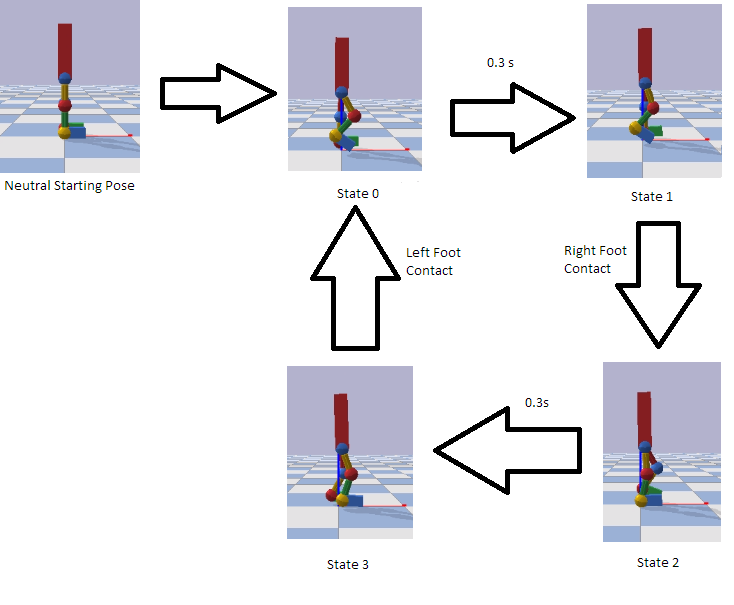
\includegraphics[scale=0.8]{finite_state}
\caption{Visual representation of the character moving through each of the four states of the finite state machine as well as the transitions between the states.}
\label{fig: finite state}
\end{center}
\end{figure}

\subsection{Torso and Swing-hip Control}
\label{subsec: torso swing hip control}
There is a natural intuition that while simulating walking it is desirable to try to keep the character's torso as upright as possible with respect to the world frame. This can be achieved by using a virtual PD controller to compute a net torso torque $\tau_{torso}$ in the world frame. It also follows that the swing  foot placement should not be affected by the current pitch of the torso. This also results in a virtual PD controller operating with respect to the world coordinates to calculate the swing hip torque $\tau_{swing}$. Since we cannot apply any external torques to the character both of these torques have to be the result of internal torques only. This can be achieved by utilizing the fact that the swing and stance hip torques ($\tau_{stance}$) are calculated separately. We can then require that the net torque seen by the torso is in fact a result of the swing and stance hip torques
\begin{equation}
\tau_{torso} = -\tau_{stance} - \tau_{swing},
\label{eqn: net torso}
\end{equation}
\noindent
and can consequently rearrange En. \ref{eqn: net torso} to calculate the torque for the stance hip. This ensures that the torques remain internal and satisfies the desired behaviour.

\subsection{Balance Feedback}
A key component to the control strategy is the balance feedback, whose aim is to try and help the character's balance as it walks. The main strategy for achieving this is to apply a feedback law that affects the placement of the swing foot. Intuitively we would like to see balance behaviour where if the character was falling forward a larger step would be taken forward and if falling backwards, a smaller step. We can achieve this by modifying the original swing hip's target angle to be dependent on the position and velocity of the torso's center of mass. This can be done by applying the following feedback term to the swing hip

\begin{equation}
\Theta_d = \Theta_{d0} + c_dd+ c_vv.
\label{eqn: balance feedback}
\end{equation}
\noindent
In this equation we calculate a new target angle for the swing hip based on the original desired angle $\Theta_{d0}$, the horizontal distance between the stance ankle and the torso's center of mass $d$, and the forward velocity of the center of mass $v$. Two more gain parameters are introduced into the model as a result of this feedback, $c_d$ and $c_v$. When the character is moving slowly $c_d$ has a more significant impact on the balance control and consequently $c_d$ is often much larger than $c_v$. Both $d$ and $v$ are needed since it is the combination of these parameters that fully describes the current position of the character. Including both allows for balance control that is responsive to the torso pitching a large distance slowly and pitching quickly but over perhaps a smaller distance. 

\subsection{Character Representation in Robotic Languages}
There are a few different options available for the format one can use to represent a character for a simulation. This project explored two: Unified Robot Description Format (URDF) XML \cite{urdf} and MuJoCo XML \cite{mujoco}. Both of these formats are supported by PyBullet for parsing/loading, and both come from sources that integrate these formats into their own physics simulators. While both of these formats accomplish the same goal of providing a representation for the character they are different in subtle ways.\\

The difference most relevant to this project is their treatment of constraining a body to 2D. In URDF you cannot specify constraints on the body in the global frame using the XML. URDF therefore places the task of constraining the body onto the physics simulator itself. This became a problem because the Bullet functionality for constraining characters is not exposed in the PyBullet implementation. PyBullet does provide some functionality for creating constraints but it is limited to prismatic, fixed, point to point, and gear joints none of which provide the desired behaviour of a hinge joint. This means it was not immediately clear how to constrain the character to 2D using URDF and PyBullet together and after a large amount of frustration it became clear that switching the character representation was the only option.\\

MuJoCo was the next choice and the format that was eventually used in this project because it allows the body to be constrained to 2D in the XML specification which PyBullet could parse in and adhere to. In the XML limits on the joints, the geometry of the links, and the masses of each link are defined. For the character used in the project the link masses are in Table \ref{tbl:link masses} and the joint limits are given in Appendix \ref{apdx: character} with the rest of the detailed code documentation.\\

\begin{table}[ht]
\caption{Link Masses}
\begin{center}
\begin{tabular}{|c|c|}
\hline
Link & Mass(kg) for each\\
\hline
Torso & 15\\
\hline
Thigh & 7\\
\hline
Shin  & 5\\
\hline
Foot & 1\\
\hline
Hips, Knees, Ankles & 0.5\\
\hline
\end{tabular}
\end{center}
\label{tbl:link masses}
\end{table}

\subsection{PyBullet and Debugging}
As mentioned in the previous section PyBullet is a python wrapper for the C++ Bullet library. As a result of this only some components of the Bullet library are available to PyBullet users. This makes it extremely difficult to find resources when trying to debug an issue or weird behaviour. Often forums will be focused on using Bullet only and the solutions provided by other users requires Bullet functionality not exposed in PyBullet. Furthermore Bullet is not popular enough that all problems encountered have solutions available online. As an example, if you make the time step of the simulation larger the character floats up off the ground and into the air, no longer adhering to the gravity or physics of the simulation. I suspect this has something to do with the integrators being unable to produce valid approximations but there was no solution or explanation of this phenomenon anywhere online. \\

Excluding obvious incorrect behaviour debugging these systems are extremely tedious and frustrating. For the most part trying to assess and understand the behaviour you are seeing in your character is done visually and through print statements. PyBullet does have some debugging capabilities such as being able to put lines and text in the GUI, as well as change the camera and visualizations. The most "useful" debugging ability is to create a slider which allows you to dynamically change a parameter. Personally I did not use any of these debugging tools since there are a large number of parameters that are all interdependent and it's easier to modify things manually. For example if you want a walk to lift the knees higher you need to modify the hip, knee, and ankle target angles simultaneously. One of the aspects of projects like this that is generally under-reported in academic papers is the amount of time that goes into manually trying to find these parameters. Debugging these systems boils down to running simulations repeatedly and trying to fine tune based off of what appeared to go wrong. Of course base starting values can be approximated by using angles that seem reasonable in the real world but all of the fine tuning is done by hand. Furthermore, the fine tuning gets more complicated when you include the more macro level parameters like $k_p$, $k_d$, $c_d$, and $c_v$. When trying to achieve the most optimal motion theses parameters can also play a huge part in the behaviour achieved. Overall, PyBullet does not seem to provide any sort of meaningful structure to make this process any easier and manually tuning parameters appears to be the most common strategy.\\

Another issue with debugging these systems is since you have a layered representation of the character in XML being loaded into the simulator, another source for issues is introduced. For example the MuJoCo representation, while better for constraining the character, was not without its' own frustrations. After constraining the body to 2D the character was exhibiting weird behaviours where its' legs would not fall to the ground if it was lying on its' back, choosing instead to stick up in the air.  This is clearly the wrong behaviour as we would expect gravity to be pulling the legs towards the ground and for the character to lie flat on the plane. It should be noted that the URDF character did not have this problem even through they were built out of the same geometries. Again there were no resources available to ascertain why the MuJoCo character was behaving strangely. After many hours of painstakingly trying to narrow down the cause of this behaviour it became apparent the only change needed was the geometry of the legs.\\
 
In the initial representation the thigh and shin segments were made out of rectangles. When these components were switched to capsules then the MuJoCo character began to behave in the same manner as the URDF one (which was still using rectangles). I believe this is due to some sort of internal collision detection that was occurring between the different leg segments in the character. This indicates that the way collision detection was being done for the MuJoCo character vs the URDF character was somehow different and it is minor details like this that are incredibly frustrating to deal with and often go undocumented.  

\subsection{Finding }

\newpage
\section{Results and Discussion}

Tables \ref{tbl: target angles} and \ref{tbl:parameters} contain the main results of this project, the target angles and parameter values used. Using these parameters the figure is capable of walking until it falls off the edge of the plane. The balance feedback helps it move but was not strenuously tested by the environment. For example the plane it walks on is flat and there are no physical obstacles that the character encounters. The values for $k_p$ and $k_d$ were selected by hand based off the fact that they allowed for large enough movement of the links to get walking behaviour. The balance feedback terms were chosen by first trying to optimize the target angles and PD parameters as much as possible and then manually tuning the balance terms such that they improved the motion. Weird behaviour is seen if the character falls or gets out of the pattern of motion. Often times the character will fall and flail about on the ground but other times the character will freeze in an odd position where it seems like neither the simulation nor gravity are actually working. As mentioned above trying to debug this problem lead to an unresolved issue with PyBullet where the simulator was behaving weirdly and I couldn't figure out how to resolve it. 
\begin{table}[ht]
\caption{Target Angles}
\begin{center}
\begin{tabular}{|c|c|c|}
\hline
State & Target Angles & Angle(rad) \\
\hline
0,1,2,3 & Torso & 0\\
\hline
\multirow{5}{*}{0,2}&Swing Hip & 0.7\\\cline{2-3}
& Swing Knee & -1.3\\ \cline{2-3}
& Swing Ankle & 0.2\\\cline{2-3}
& Stance Knee& -0.05\\\cline{2-3}
&Stance Ankle & 0.2\\\cline{2-3}
\hline
\multirow{5}{*}{1,3}&Swing Hip & -0.7\\\cline{2-3}
& Swing Knee & -0.05\\ \cline{2-3}
& Swing Ankle & 0.2\\\cline{2-3}
& Stance Knee& -0.1\\\cline{2-3}
&Stance Ankle & 0.2\\\cline{2-3}
\hline
\end{tabular}
\end{center}
\label{tbl: target angles}
\end{table}

\begin{table}[ht]
\caption{Parameters}
\begin{center}
\begin{tabular}{|c|c|c|}
\hline
State & Parameter & Value \\
\hline
0,1,2,3 & $k_p$ & 800 Nm/rad\\
\hline
0,1,2,3 & $k_d$ & 80 Nm/rad\\
\hline
\multirow{2}{*}{0,2}& $c_d$ & 0\\\cline{2-3}
& $c_v$ & 0.2\\ \cline{2-3}
\hline
\multirow{2}{*}{1,3}& $c_d$ & 2.2\\\cline{2-3}
& $c_v$ & 0\\ \cline{2-3}
\hline
\end{tabular}
\end{center}
\label{tbl:parameters}
\end{table}


\begin{figure}
\begin{center}
\includemedia[
  width=\linewidth,
  height=\linewidth,
  activate=pageopen,
  addresource=walking2.mp4,
  flashvars={source=walking2.mp4}
]{}{VPlayer.swf}
\caption{Video demonstrating the character walking on the plane.}\label{vid: character walking}
\end{center}
\end{figure}



\begin{figure}
\begin{center}
\includemedia[
  width=\linewidth,
  height=\linewidth,
  activate=pageopen,
  addresource=falling.mp4,
  flashvars={source=falling.mp4}
]{}{VPlayer.swf}
\caption{Video demonstrating what happens when the character falls and displays erratic behaviour.}\label{vid: character falling}
\end{center}
\end{figure}

\section{Conclusion}

In conclusion this project shows that the SIMBICON framework can be reimplemented in a newer physics simulator with the same results. Further it shows that the techniques for creating a biped that moves in two dimensions in a stable, balanced way are valid and an excellent place to start in building more complex motions in higher dimensions. 
 
\section{Further Works}
The simple biped locomotion control presented in this paper can easily be expanded into many avenues for further works. The first and most obvious of which is to control the motion in 3D instead of the 2D model presented here. Removing the constraint on the body would introduce another dimension of balance control that would need to be implemented and optimized, allowing for steps to the side to help keep the figure upright. When working with this 2D model one could use optimization routines to try and find the set of parameters which produces the longest upright walking time. Stochastic policy search, cyclic coordinate decent and covariance matrix adaptation are all methods that could be applied to finding the particular balance parameters, $c_d$ and $c_v$ for optimal walking. Another expansion of this model is different gaits and walking terrain. For example running, walking with high knees, jumping, and even more complex movements could be implemented using the finite state machine framework. Furthermore inclined or bumpy terrain as well as external forces acting on the body could be used to further push the balance and locomotion control. Finally models like these can be used to bridge the gap between simulation and reality. The locomotion control can be applied to real life robots and these models can help guide the way in which their locomotion is developed. 

\newpage
\bibliography{thesisBib}{}
\addcontentsline{toc}{section}{References}\bibliographystyle{ieeetr}
\newpage

\appendix
\section{Code and Documentation: Character Representation}
\label{apdx: character}
\subsection{MuJoCo XML code}
\lstset{breaklines=true,breakatwhitespace = false, basicstyle=\footnotesize, numbers=left}
\lstinputlisting[language=xml]{../../legs.xml}
\subsection{Character Representation Documentation}
Lines 8-10 are the most important in this representation since they are the ones that constrict the body to 2D. Here we construct the contraint out of three separate joints, one for each dimension. Along the x and z axis the worldbody is constrained with a slide joint, which gives the worldbody one degree of freedom along each axis, which results in unconstrained motion in the 2D x,z plane. Along the y axis we constrain the worldbody to a hinge joint, which gives the worldbody one degree of rotational freedom around the y axis. The overall effect of these joint constraints is that the worldbody is constrained to 2D motion where it can still fall forward and backward but not to the sides. \\

MuJoCo uses a nested representation to define their kinematic tree of parent/child relationships. Here the parent/child relationship is enforced by the child relationship already present in XML. So to be a child of a link means you must be a child of your parents' link tag, which means you must be a nested XML element. In this way we can define two children to be at the same level, for example left and right hips, while still allowing each of those children to have children of their own, for example left and right thighs. In contrast to URDF where each link is defined separately and you must specify joints to link them together, if no joint is specified between a parent and its' child a fixed joint is generated by default.  At the highest level is the worldbody which in our case is the torso, now constrained to 2D, and is the only part of the character that exists in relation to the world frame directly.\\

The \verb; <joint>; tag: In this tag we can define which axis the rotation occurs around and where the joint is located. It is here that we also limit the joints, with the joint limits given in degrees. The limits were selected to mirror the true limits those joints experience on the human body. \\

The \verb; <geom>; tag: here we finally define the geometries that make up the visual components of the character. It is very important to note that capsules must be used to make up the main portions of the legs rather than rectangles. Initially they were made of rectangles and there was very weird behaviour in the legs due to internal collisions between the legs and sphere "joints" which were only resolved when the geometry was changed. The feet could however remain rectangles since they did not seem to experience this behaviour.\\ 




\section{Code and Documentation: Main Program}
\label{apdx: main program}
\subsection{Python Code}
\lstinputlisting[language=Python]{../../finiteState.py}

\subsection{Main Program Documentation}

Throughout this piece of code \verb;getJointState(legsID, joint_index); returns an array of which we are interested in: index 0: the current velocity of the queried joint, and index 1: the current position.\\

The first 15 lines of code are necessary for loading the character and plane in as MuJoCo and URDF files respectively. As well as starting the legs slightly above the ground otherwise it loads the character midway through the plane and you have weird contact collisions happening right at the beginning of the simulation which cause the character to fly upwards erratically. Finally we start the camera perpendicular to the character to better see its' motion when walking.\\

Lines 21-31 are static values for the link and joints labels needed for the simulation. Figures \ref{fig: link labels} and \ref{fig: joint labels} show how these are labelled for the character used. These values can be determined dynamically by iterating over all values from 0 to getNumJoints(legsID) and calling getJointInfo() for each joint, or getLinkState() for each link although in the link case there is no way to get the total number of links in the character. I determined these values via guessing and checking and decided to simply store them statically since the character's representation does not change. \\

Lines 33-54 are all the parameters needed to run the simulation, they are stored in variables so that modifying them is easy as there is only one place in the code to change the values. The parameters correspond to the values in Tables \ref{tbl: target angles} and \ref{tbl:parameters}.\\

Lines 56-59 contain parameters used in the simulation. The time step is used by the integrators and the $foot\_contact\_tol$ is used as a tolerance value for determining if a foot has made contact with the plane.\\

\verb;def stance_leg_torque(swing_hip_torque); is the first helper function whose job is to calculate the torque for the stance hip using the method discussed in Subsection \ref{subsec: torso swing hip control} and the implementation closely follows Equation \ref{eqn: stance hip torque}. \\

\verb;def balance_feedback(target_angle, stance_ankle_link, cd,cv); in this helper function we are computing the balance feedback as given in Equation \ref{eqn: balance feedback}. Here we approximate d by the difference in the x coordinates of the base and the ankle's center of mass as the positions are given in 3D coordinate space. \\

\verb; def in_contact(contact_points, contact_links); this is a simple helper function who takes in a list of links currently in contact with the plane and outputs true if any of the links are are interested in ($contact\_links$) is in contact with the plane. This function is used to determine if the foot or ankle is in contact with the plane for states 1 and 3.\\

\verb; def set_torques_0(); is the main function in charge of calculating and setting all the torques for state 0.\verb; def set_torques_1(), def set_torques_2(); \verb;def set_torques_3(); perform the same functions for their respective states so for brevity only state 0 will be talked about in depth. Torques are calculated for each of the joints by getting the current state of the joint and using Equation \ref{eqn: pd control}. The final steps are to update the torques being applied to the various joints and stepping the simulation to apply them.\\

\verb; def state0() def state2(); these two functions control the finite state machine for states 0 and 2. In these states the transition to the next state is based on an interval of time passing. During this time, the torques are repeatedly updated to move the character.\\

\verb; def state1() def state3(); these two functions control the finite state machine for states 1 and 3. In these states the state transition is governed by the foot making contact with the plane. Here we check to see if either the ankle or the foot is in contact with the plane and if yes we move on to the next state, otherwise we keep updating the torques. We check for both the ankle and the foot since there were issues with it not always recognizing the foot was in contact with the ground. These states are ones in which the simulation often gets stuck since it will continuously wait for the foot contact which doesn't always occur.\\

Line 264-267 Finally we are at the point in the program where the finite state machine is started. There is a small loop before we call \verb;state0();. This is to allow the character to fall until it comes in contact with the plane. This is because we initialized the character to load in above the plane, however if we immediately start the walking process while the character is in the air it has the potential to land on the ground in a funny position and the entire walking cycle is thrown off.


\begin{figure}
\begin{center}
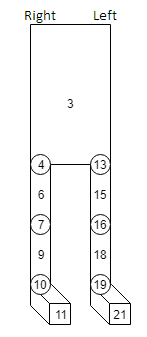
\includegraphics[scale=0.8]{link_labels}
\caption{Diagram of how the links are labelled on the character.}
\label{fig: link labels}
\end{center}
\end{figure}

\begin{figure}
\begin{center}
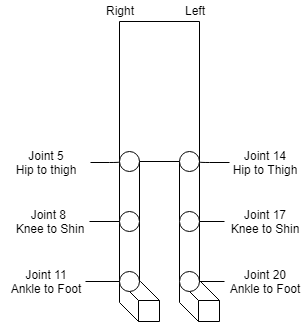
\includegraphics[scale=0.8]{joint_labels}
\caption{Diagram of how the joints are labelled on the character.}
\label{fig: joint labels}
\end{center}
\end{figure}


\end{document}